\chapter{Background}
\label{chapter:background} 



\section{DDoS attack and defense mechanisms}
\label{sec:BGDDoS}

A denial-of-service attack is characterized by an explicit attempt by attackers to prevent the legitimate users of a service from using that service~\cite{dosCert} provided by a network or server. There are two manner to launch this kind of attack. The first approach is overwhelm the network and occupy all the resources of a service sending massive volumes of useless traffic

\section{OpenFlow}
\label{sec:BGOpenFlow}

The explosion of mobile devices, server virtualization, security problems and advent of cloud service are among some of the reason that the networking industry is beginning to question the traditional network architecture. OpenFlow is intended to solve the problem of assigning resources to users in a easy-way giving them the control plane of the network without disturbing the traffic flows. 

\par 

In traditional routers or switches, both control plane (high level routing decisions) and data plane (packet forwarding) are embedded in the same device. An OpenFlow Switch separate these two functions (Figure~\ref{fig:OpenFlowSwitch}). The data plane function still resides on the switch, while the control plane is moved to a separate device called Controller (see~\ref{subsec:OFController}) that manage the switch and communicate to each other over the Secure Channel (see~\ref{subsec:SCSecureChannel}) via the OpenFlow protocol (see~\ref{subsec:OFProtocolSC}).

\par 

\begin{figure}[htb]
\centering
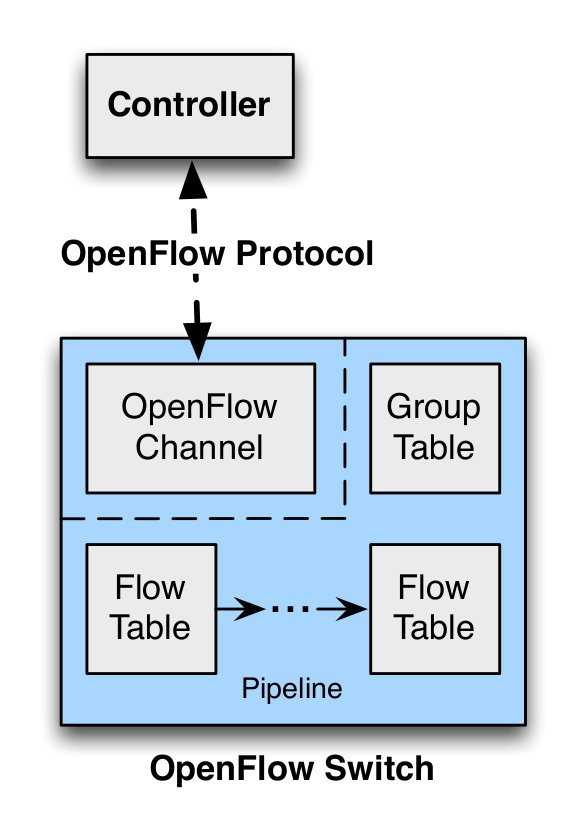
\includegraphics[width=0.5\textwidth]{./images/OpenFlowSwitch.jpg}
\caption{OpenFlow Switch components} \label{fig:OpenFlowSwitch}
\end{figure}

\par 




\par 

The firs version of the OpenFlow (1.1) protocol was released on 2011, and one year later, in February 2012, the ONF approved and published the version 1.2. Nowadays, the current version of the protocol and the one that will be used in this project is the 1.4.

\subsection{Switch Components}
\label{subsec:PFSwitchComponents}

\subsubsection{Flow Table}
\label{subsec:SCFlowTable} 

\subsubsection{Secure Channel}
\label{subsec:SCSecureChannel}

\subsubsection{OpenFLow Protocol}
\label{subsec:OFProtocolSC}

\subsection{Controller}
\label{subsec:OFController}

\section{POX}
\label{sec:BGPOX}
